\chapter{任意桌面文本输入方法}
% 手机传感信号和点击识别
\label{cha:sensing} 
本章首先详细介绍了手机传感信号的处理,包括声音和深度图像,然后在此基础上介绍了点击识别算法流程。最后描述了如何使用模拟的方法探究用户输入意图推理算法。第~\ref{cha:intro}~章中已经提到本工作主要是基于iPhone 11,因此本章中描述的参数主要适用于iPhone 11,如果将同样的算法移植到其他平台上可能需要对其做一定的调整,但并不影响算法的原理。

\section{技术原理}
\subsection{声音信号的处理}
手机的声音信号为线性PCM编码格式,采样率44100Hz。软件得到的是47Hz,每次940帧的数据流,程序需要从此数据流中识别出用户触发的点击。一次点击的声音特征一般比较明显,通常持续时间较短并且伴随峰值。另外,除去响度较大的杂音,点击峰值明显高于环境中的其他噪音。图~\ref{fig:sound-comp}~给出了某次用户点击前后声音波形图的对比。

\begin{figure}[h]
  \centering%
  \subcaptionbox{无点击的声音波形} %标题的长度,超过则会换行,如下一个小图。
    {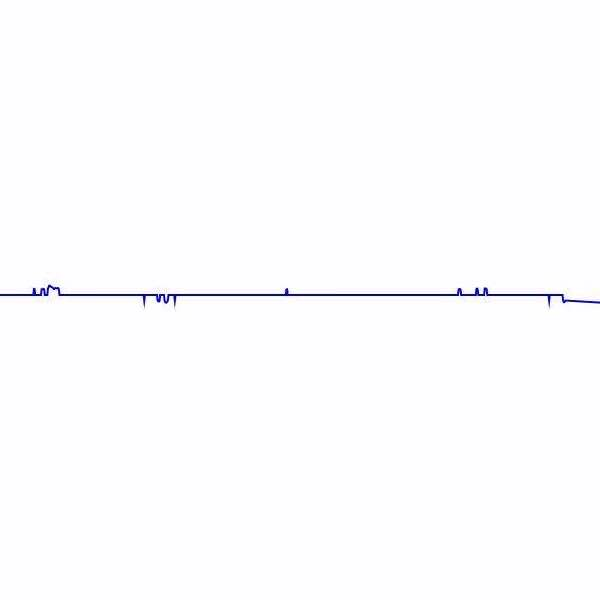
\includegraphics[height=4cm]{sound1.jpeg}}%
  \hspace{4em}%
  \subcaptionbox{某次点击的声音波形}
      {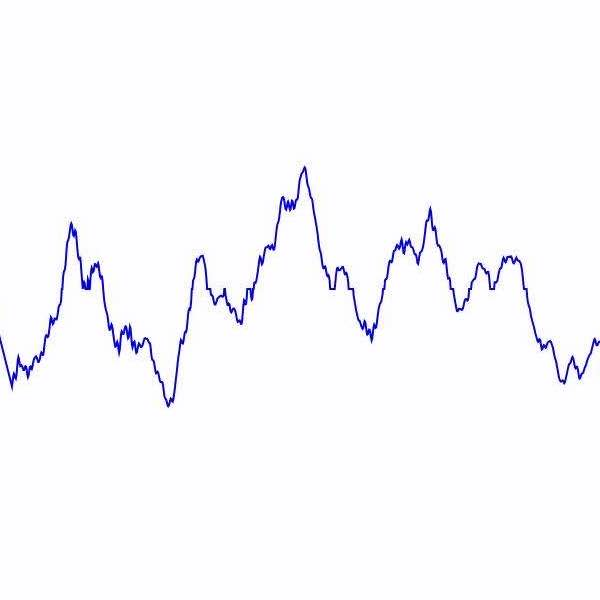
\includegraphics[height=4cm]{sound0.jpeg}}
  \caption{有无点击的声音波形对比}
  \label{fig:sound-comp}
\end{figure}

可以看出,正常无点击时波形较平,环境噪音只有很小的干扰。但是发生点击时,波峰波谷十分明显。因此,可以通过计算在一段时间窗口内数据流中超过某个阈值的数据个数判断是否有潜在的点击发生。

每帧的数据为两个字节,根据经验,周围声音的响度一般低于1000,正常点击的峰值会大于3000,因此最终的阈值设置为3000。此外,为了减少误识别,两次点击的最小间隔被设置成50ms。通过预实验,发现除了环境中有十分类似点击的其他声音外,正常情况下该阈值的设定能够准确地识别用户的点击。

\subsection{深度数据的处理}
深度数据是支持此项工作的核心,手机前置摄像头提供的深度数据大大增加了在任意桌面上进行文本输入的可能性。

手机提供的深度数据为30Hz,维度为640*480的深度图像,其中每个像素点的数值代表手机前置摄像头离该点的距离。图~\ref{fig:depth1}中展示了用户端坐在手机前的原始的深度图像,在该图中,使用肉眼即能够较为明显地分辨出用户上身的轮廓,包括双手、头部等以及环境中其他物体。其中,距离近的物体在图中黑色更显著,例如双手。

使用距离能够较容易去除图像后景等无关的信息,只剩下用户的手部。由于用户手部距离手机的位置一般为20cm-30cm,因此只有15-40cm范围的图像信息被保留下来,据此对原图加以处理后得到的图像为~\ref{fig:depth2},可以看到,用户的手部被十分完好的保存了下来,而其他的部分则被过滤了。
\begin{figure}[h]
  \centering%
  \subcaptionbox{原始深度图像\label{fig:depth1}} %标题的长度,超过则会换行,如下一个小图。
    {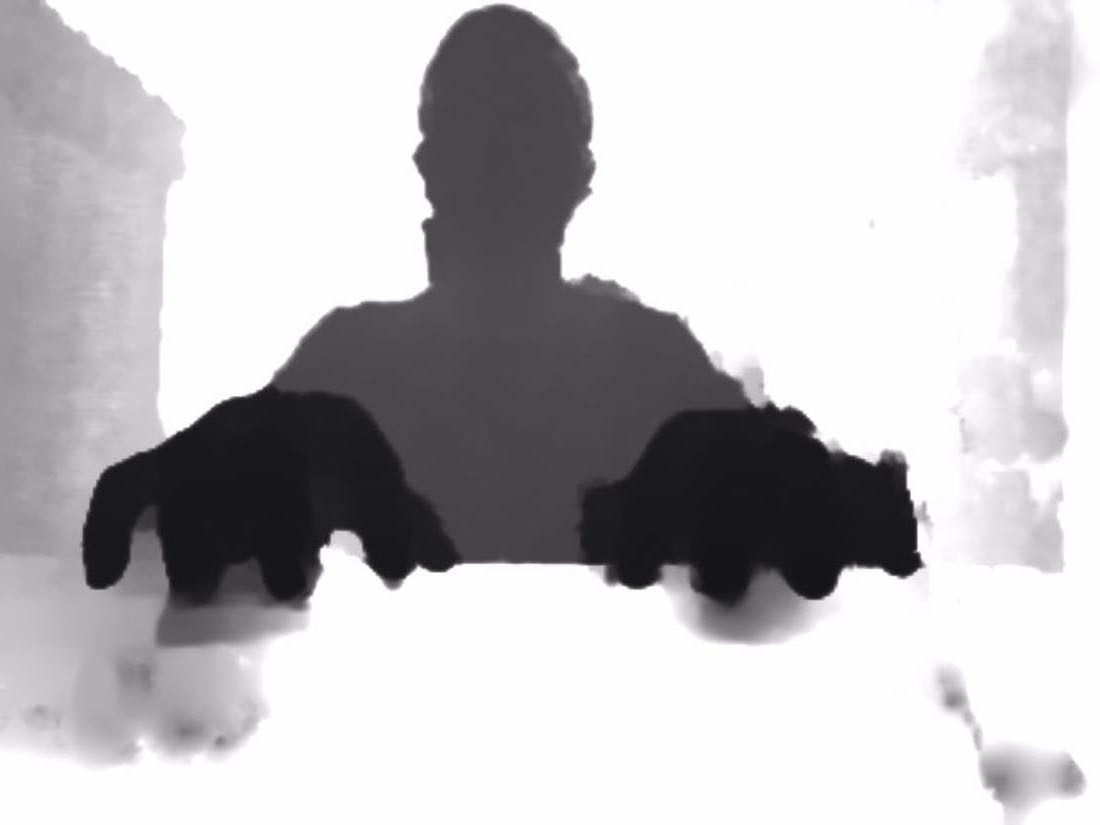
\includegraphics[height=4cm]{depth0.jpeg}}%
  \hspace{4em}%
  \subcaptionbox{处理后的深度图\label{fig:depth2}}
      {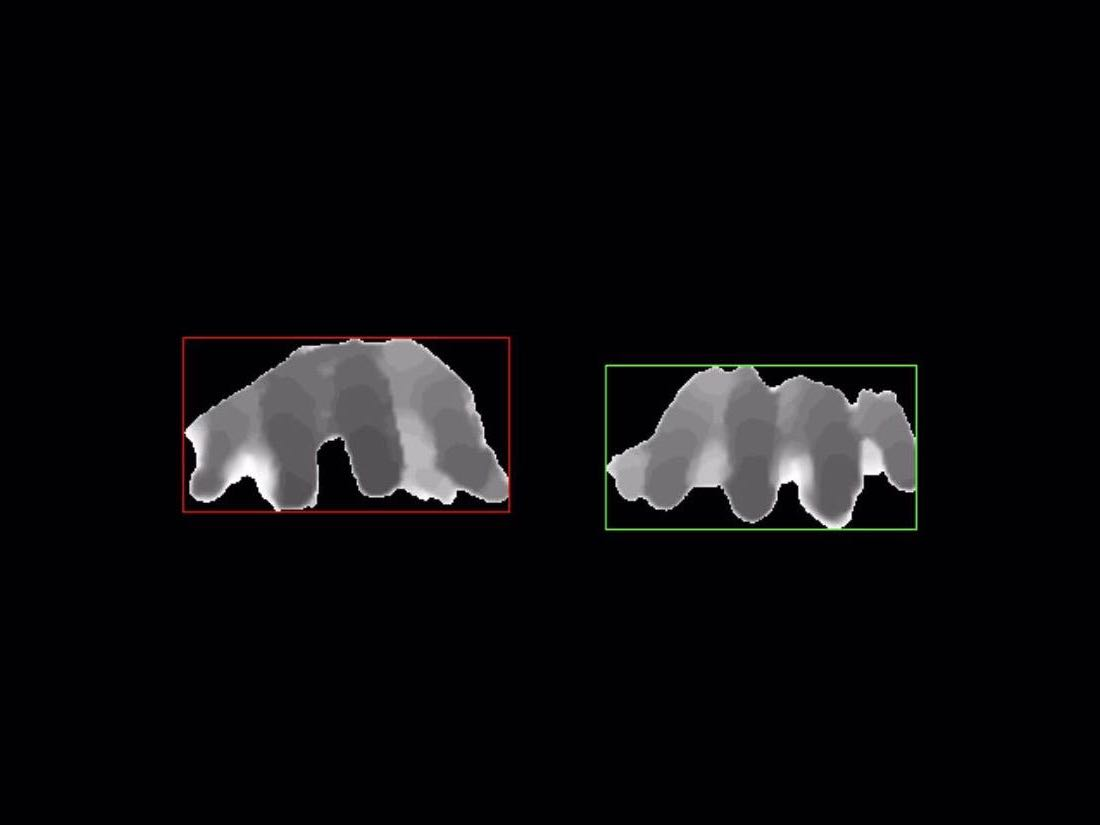
\includegraphics[height=4cm]{depth1.jpeg}}
  \caption{处理前后的深度图像}
  \label{fig:depth-image}
\end{figure}

获取处理之后的深度图像,程序首先识别出图中所有的轮廓,其中面积最大的两个即为用户的手部。当用户手部从悬浮状态发生点击时,点击的手指会位于深度图像最低点。基于这一事实,当通过声音检测到点击的瞬间,程序将首先寻找手部轮廓和轮廓外接矩形的最低点。

在图中找到最低点后,接下来便是计算点击位置离手机的距离。根据尝试,由于指缝等的干扰,直接在深度图中读取点击处的像素深度可能会出现一定的误差,因此实际的点击距离使用对该位置邻域进行洪范后的平均值作为代替。如果出现识别出多个切点的情况,距离最近的一个会被选做点击位置。

此外,基于深度图像的信息,不仅双手能够被区分,同时手部的运动状态也能够较好被监控,系统在此基础上提供了左手左移、右手右移和任意手上移的手势。
%ring queue
%手指识别

\subsection{三维坐标的计算}
前面部分已经提到了如何计算点击和手机的距离,本节将介绍如何进一步计算该点击在物理世界中的三维坐标。

相机的成像,简言之,指的是将现实世界三维空间中的点映射成为图片中二维空间中的点这一过程,即将世界坐标系中的三维坐标转化为像素坐标系的二维坐标。其原理可以用式~(\ref{imageform})表示。
% 为了获得该过程的映射关系,一般需要引入以下几个坐标系:
% \begin{itemize}
%     \item \textbf{世界坐标系:}指的是物体在三维世界中的位置,一般由相机指定,用$(U, V, W)$表示
%     \item \textbf{相机坐标系:}以相机的光心为坐标系原点,到成像平面的距离为焦距,可由世界坐标系旋转和平移得到,用$(X, Y, Z)$表示
%     \item \textbf{图像坐标系:}在成像平面上的二维坐标系,用$(x, y)$表示
%     \item \textbf{像素坐标系:}最终图片的像素坐标,也在成像平面上,由图像坐标系平移和缩放得到,用$(u, v)$表示
% \end{itemize}

\begin{equation}
    \label{imageform}
    \begin{aligned}
    \begin{bmatrix}
        u \\
        v \\
        1
    \end{bmatrix}
    &= \frac{1}{Z} \begin{bmatrix}
        f / s_x & 0 & o_x & 0\\
        0 & f / s_y & o_y & 0 \\
        0 & 0 & 1 & 0
      \end{bmatrix}
      \begin{bmatrix}
        R & t \\
        0^{T} & 1
      \end{bmatrix}
      \begin{bmatrix}
        U \\
        V \\
        W \\
        1
      \end{bmatrix} \\
    &= \frac{1}{Z} \begin{bmatrix}
        f / s_x & 0 & o_x & 0\\
        0 & f / s_y & o_y & 0 \\
        0 & 0 & 1 & 0
      \end{bmatrix}
      \begin{bmatrix}
        X \\
        Y \\
        Z \\
        1
      \end{bmatrix}
    \end{aligned}
\end{equation}

式~(\ref{imageform})中的$(X, Y, Z)$为需要计算的点击在物理世界中的坐标,而$(u, v)$则是前文获得的点击在深度图像中的位置。$f$,$s_x$,$s_y$,$o_x$,$o_y$,$R$,$t$都属于相机的参数,可通过对应接口获取。

前文的章节已经提到了如何获取点击位置在世界坐标系中的深度坐标$Z$。此外,在实验设备中,相机坐标系和世界坐标系只是将$X, Y$调换为$V, U$。因此,前述的公式可以化简为公式~(\ref{equ:world-coord})。这样,一次点击的全部三维信息即能够全部获得。由于在实际使用时手机靠于墙壁,和桌面垂直,即$Y$方向垂直桌面,因此$Y$坐标基本为定值。后文中主要用到$X$和$Z$方向坐标,为了表述方便,仍然将其称之为横轴和纵轴。
\begin{equation}
  \begin{aligned}
  X &= \frac{(u - o_x)s_x}{f_x} \times Z \\
  Y &= \frac{(v - o_y)s_y}{f_y} \times Z
  \end{aligned}
  \label{equ:world-coord}
\end{equation}

\section{点击识别算法}
整个点击识别的算法的框架以本章前面部分描述的声音信号和深度图像处理的内容为基础。算法在接收到声音数据后,如果此时双手在合适位置,并且声音达到阈值,则识别到点击发生。然后,在当前时刻对应的深度图像中,寻找到手部最低点作为点击位置,并计算出其三维坐标,即为点击发生位置的坐标。经过前期的预实验,用户在点击时需要使用一定力度,如果敲击过轻则为不合法点击,排除了在一般触摸屏上输入时因为无意触碰造成误识别的情况。此外,算法同时会检测是否识别到用户的手势。

算法的伪代码表述如下:
\begin{algorithm}[h]
  \caption{点击识别算法伪代码} %算法的名字
  \hspace*{0.02in} {\bf Input:} %算法的输入, \hspace*{0.02in}用来控制位置,同时利用 \\ 进行换行
  声音数据流、深度数据流\\
  \hspace*{0.02in} {\bf Output:} %算法的结果输出
  点击的世界坐标
  \begin{algorithmic}[1]
  % \State some description % \State 后写一般语句
  \If{Tap Detected}
    \If{Hands in Range}
      \If{Gestures Detected}
        \State Process gestures
      \Else
        \State Find the tangent point of hand contour and its bounding box
        \State Calculate the tap coordinate in world coordinate system
        \State \Return tap coordinate
      \EndIf
    \Else 
      \State Marked as invalid tap 
      \State \Return
    \EndIf
  \EndIf
  % \For{condition} % For 语句,需要和EndFor对应
  %   \State ...
  %   \If{condition} % If 语句,需要和EndIf对应
  %     \State ...
  %   \Else
  %     \State ...
  %   \EndIf
  % \EndFor
  % \While{condition} % While语句,需要和EndWhile对应
  %   \State ...
  % \EndWhile
  % \State \Return result
  \end{algorithmic}
\end{algorithm}

\section{用户输入意图推理算法}
本节中通过第~\ref{cha:exp1}~章中实验收集的用户在桌面上的点击数据进行模拟实验,试图探究能够准确预测用户输入单词的推理算法。

对于每一种算法,模型的输入为用户的点击位置信息,输出为该算法预测出的概率最高的五个可能的单词。然后将其与正确的单词进行比对,分别计算对应的概率第一高到概率第五高的单词级别准确率。在模拟时,本文使用了美国国家语料库\cite{anc},其中收录了各种正式和非正式场景下使用的总计2,000多万个单词。从该语料库中本文进一步挑选了出现频率最高的10,000个单词作为词库,在计算时将频率作为单词出现概率,同时保证了用户在上个实验中输入的所有单词都出现在词库中。

\subsection{算法选择}
文献综述部分提到虚拟键盘上通常使用的纠错算法大部分都是基于贝叶斯原理,包括绝对位置和相对位置两种形式。相对位置的纠错算法也有两种形式,一是当一只手或者一个手指负责整个键盘时,研究者直接计算两次点击的位置变化;二是当用户使用两只手输入时,通常将两手的位置变化分开考虑,即计算一个单词的出现概率时,将一连串点击归类为左右手分别计算,最后相乘。然而,用户在十指盲打时,尤其是在本项研究的使用场景中是双手抬起,两只手的运动是一个整体,可能并不相互独立,因此本文试图探索其是否可能呈现第一种相对位置运动规律,即运算时直接计算连续点击的位置变化。从而本文一共探究了三种推理算法,分别称为绝对模型、全键盘相对模型(第一种形式)、半键盘相对模型(第二种形式)。使用公式~(\ref{equ:fitkeyboard})~对三种点击模型进行拟合,如果是相对模型,则将式中$x$,$y$,$\textbf{X}$,$\textbf{Y}$换成相对变化量。表~\ref{tab:modelr2}~的结果显示所有的点击模型拟合$R^2$都超过了0.80,并且相对模型下对于纵轴的拟合效果更好,说明用户在纵轴的点击规律更符合相对模型。在计算相对模型时,若出现对应的位置变化未在用户数据中出现,则仍然使用绝对模型进行计算。

\begin{table}[htb]
  \centering
  \begin{minipage}[t]{0.6\linewidth} % 如果想在表格中使用脚注,minipage是个不错的办法
  \caption[三种点击模型拟合的$R^{2}$]{三种点击模型拟合的$R^{2}$}
  \label{tab:modelr2}
    \centering
    \begin{tabularx}{\linewidth}{cccc}
      \toprule[1.5pt]
      %  & \multicolumn{2}{c}{总体}&\multicolumn{2}{c}{左手} &  \multicolumn{2}{c}{右手} \\\midrule[1pt]
      & 绝对模型 & 全键盘相对模型 & 半键盘相对模型 \\\midrule[1pt]
      X & 0.96 (0.01) & 0.95 (0.01) & 0.82 (0.02) \\
      Y & 0.85 (0.01) & 0.89 (0.01) & 0.91 (0.02) \\
      \bottomrule[1.5pt]
    \end{tabularx}
  \end{minipage}
\end{table}

此外,对于每一种点击模型,本文计算了单人和整体两种情况下的准确率。其中单人指的是将每个人的落点分别计算准确率后计算平均值,整体指的是将所有人的落点合并并且平移后计算总准确率。在实际使用中,因为一开始缺乏用户个性化的数据,所以总是从整体出发。每一种模型都测试了676个单词,因此总共测试了4,056个英文单词。

\subsection{模拟结果}
不同情况下的准确率模拟结果如图~\ref{fig:simulation}。可以看到,概率最低的为整体下使用全键盘相对模型,但预测概率最高的单词是正确的概率仍然接近80\%,说明这几个模型的预测效果都较为良好。同一个模型而言,单人的情况总是好于整体,因为每个人的点击规律并不相同,将按键平移合并后会增加不准确性,从而降低预测准确率。但是因为实验中人数较少,单人和整体的差距不是十分明显。

\begin{figure}[h] % use float package if you want it here
    \centering
    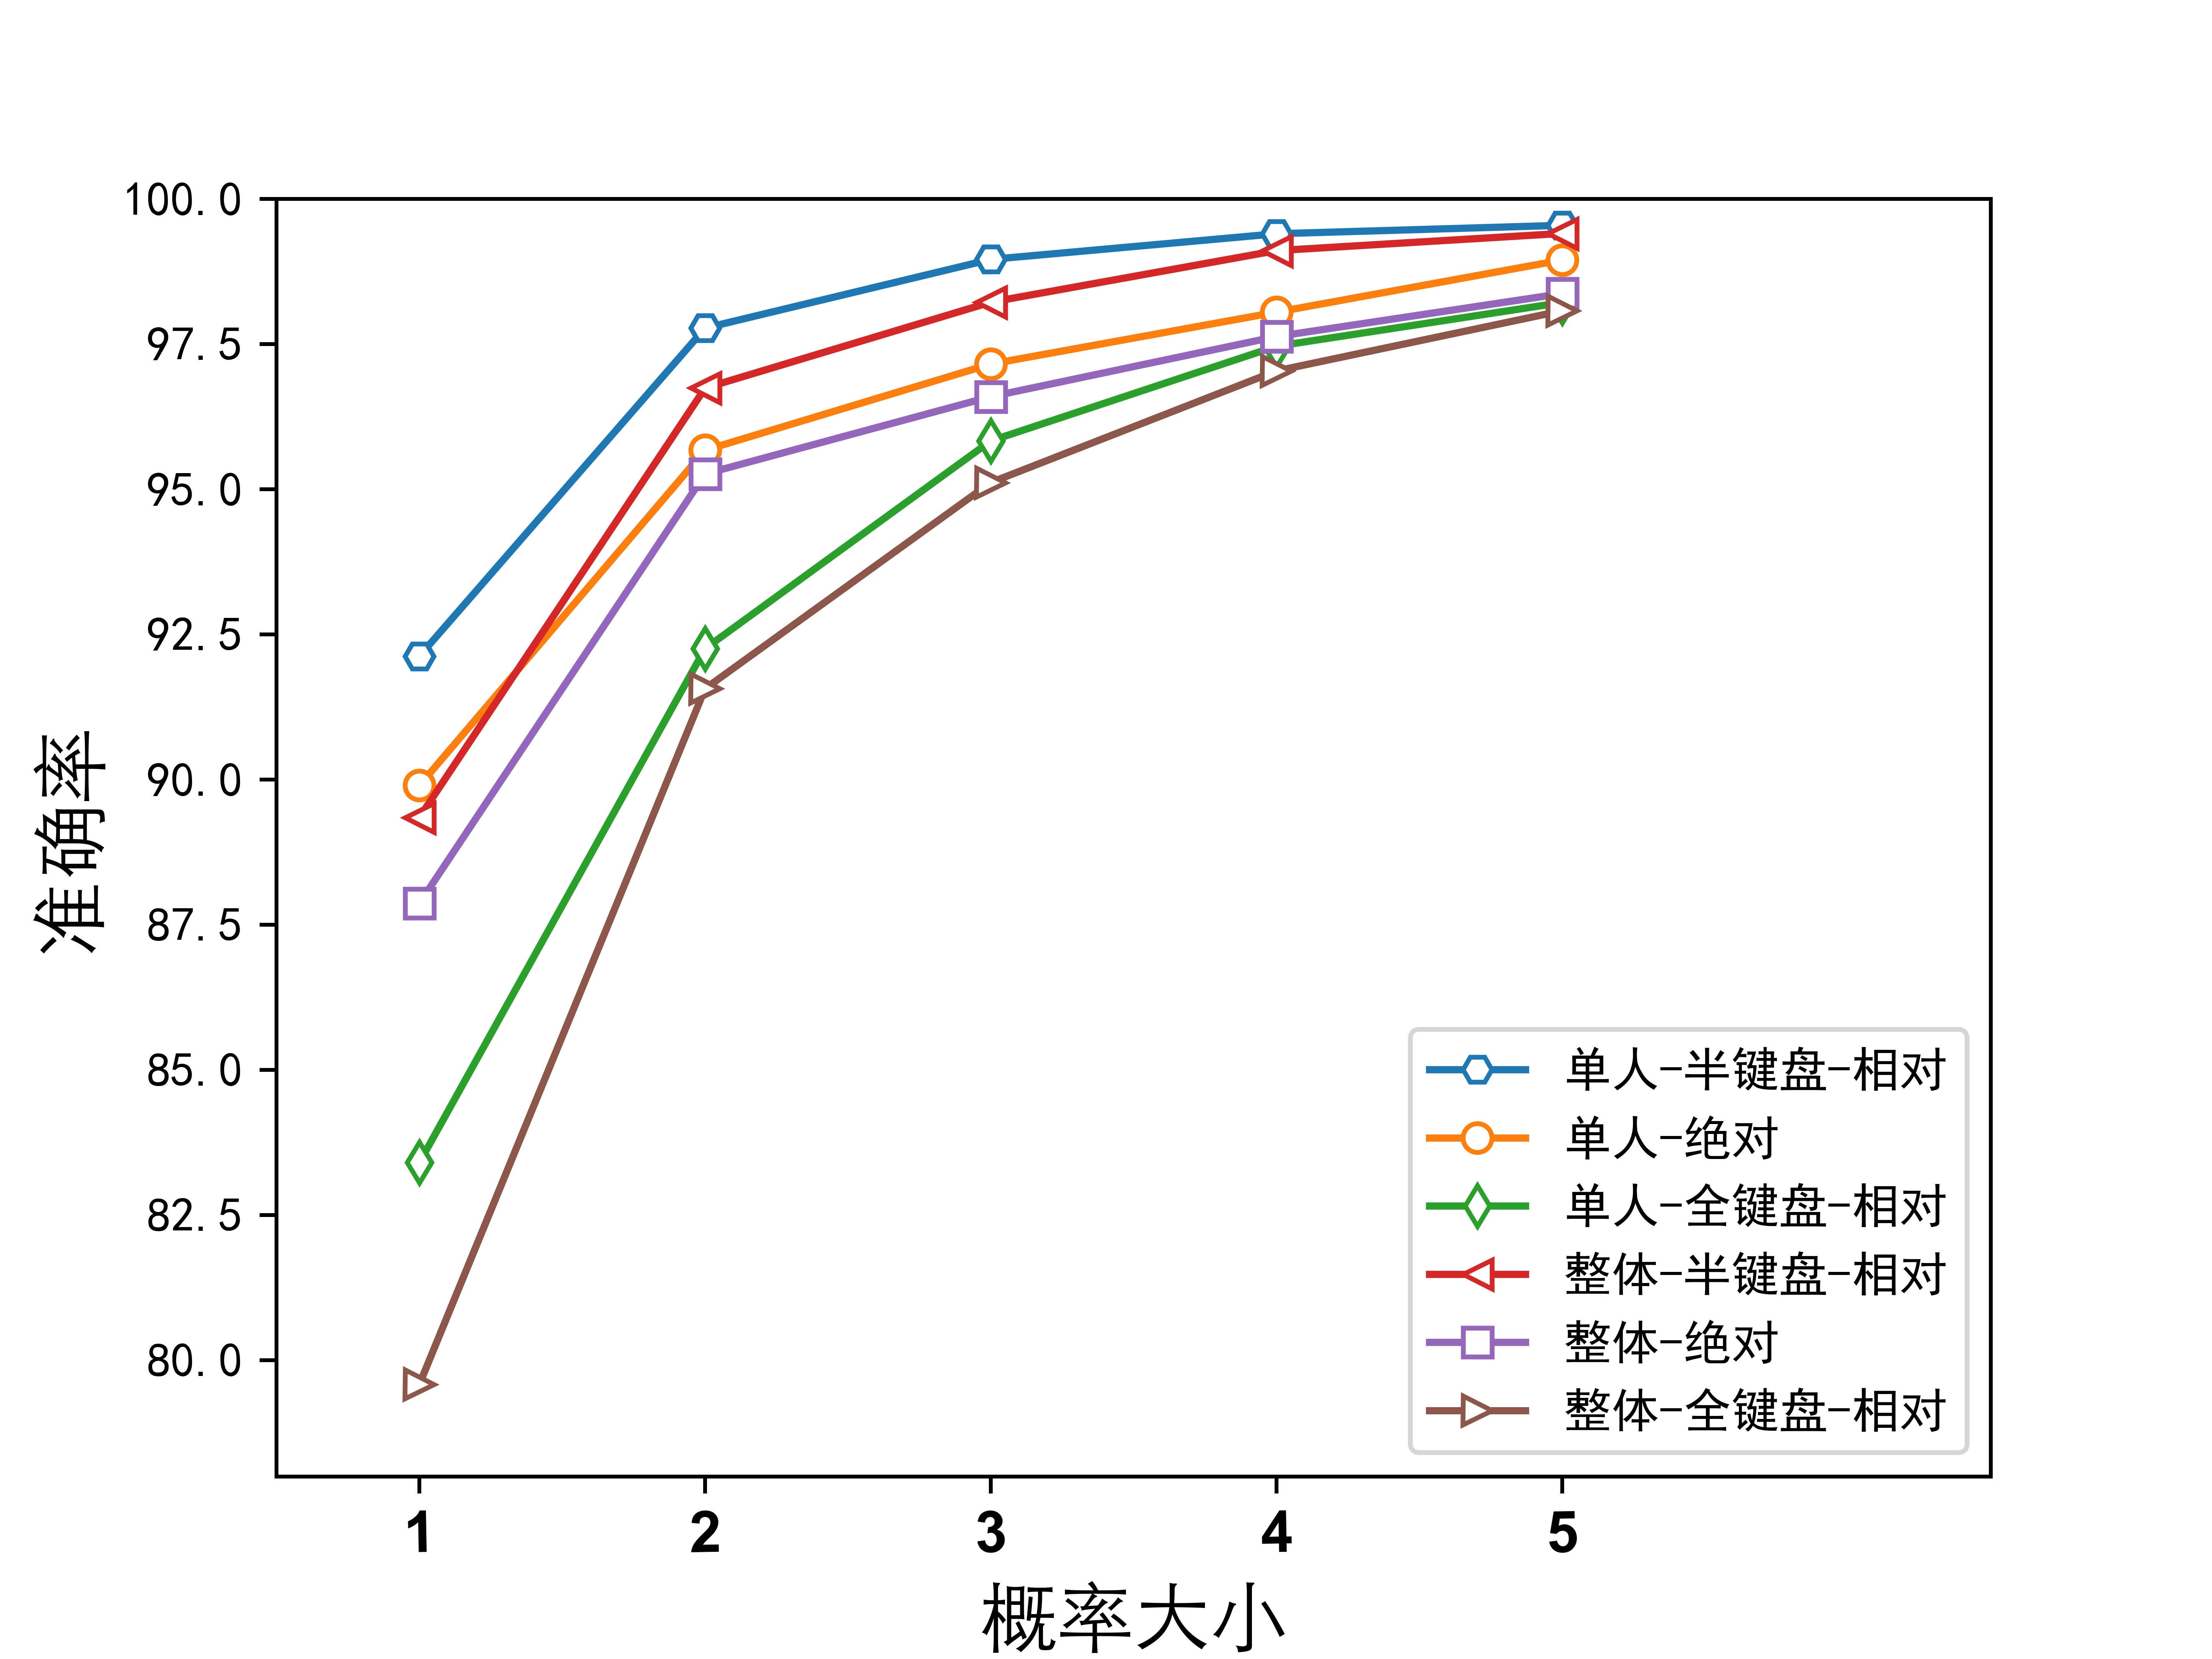
\includegraphics[width=10cm]{figures/acc.jpg}
    \caption{不同算法模拟的准确率}
    \label{fig:simulation}
\end{figure}

无论是在单人和整体的情况下,模型的准确率从大到小排序均为半键盘相对模型、绝对模型、全键盘相对模型。说明用户在桌面上十指输入时更符合两只手独立分别运动的规律。绝对模型能够较好拟合用户落点,说明用户点击时能够明显区分不同的按键,半键盘的相对模型能够减少用户点击的误差,从而能够进一步提高准确率。综合考虑,本项工作选择半键盘相对模型作为单词输入推理算法。